% This is "sig-alternate.tex" V2.1 April 2013
% This file should be compiled with V2.5 of "sig-alternate.cls" May 2012
%
% This example file demonstrates the use of the 'sig-alternate.cls'
% V2.5 LaTeX2e document class file. It is for those submitting
% articles to ACM Conference Proceedings WHO DO NOT WISH TO
% STRICTLY ADHERE TO THE SIGS (PUBS-BOARD-ENDORSED) STYLE.
% The 'sig-alternate.cls' file will produce a similar-looking,
% albeit, 'tighter' paper resulting in, invariably, fewer pages.
%
% ----------------------------------------------------------------------------------------------------------------
% This .tex file (and associated .cls V2.5) produces:
%       1) The Permission Statement
%       2) The Conference (location) Info information
%       3) The Copyright Line with ACM data
%       4) NO page numbers
%
% as against the acm_proc_article-sp.cls file which
% DOES NOT produce 1) thru' 3) above.
%
% Using 'sig-alternate.cls' you have control, however, from within
% the source .tex file, over both the CopyrightYear
% (defaulted to 200X) and the ACM Copyright Data
% (defaulted to X-XXXXX-XX-X/XX/XX).
% e.g.
% \CopyrightYear{2007} will cause 2007 to appear in the copyright line.
% \crdata{0-12345-67-8/90/12} will cause 0-12345-67-8/90/12 to appear in the copyright line.
%
% ---------------------------------------------------------------------------------------------------------------
% This .tex source is an example which *does* use
% the .bib file (from which the .bbl file % is produced).
% REMEMBER HOWEVER: After having produced the .bbl file,
% and prior to final submission, you *NEED* to 'insert'
% your .bbl file into your source .tex file so as to provide
% ONE 'self-contained' source file.
%
% ================= IF YOU HAVE QUESTIONS =======================
% Questions regarding the SIGS styles, SIGS policies and
% procedures, Conferences etc. should be sent to
% Adrienne Griscti (griscti@acm.org)
%
% Technical questions _only_ to
% Gerald Murray (murray@hq.acm.org)
% ===============================================================
%
% For tracking purposes - this is V2.0 - May 2012

\documentclass{sig-alternate-05-2015}
\usepackage{color}
\usepackage[colorlinks=black,
            linkcolor=blue, 
            anchorcolor=blue,
            citecolor=red
            ]{hyperref}
\usepackage{longtable}

\begin{document}

% Copyright
%\setcopyright{acmcopyright}
%\setcopyright{acmlicensed}
%\setcopyright{rightsretained}
%\setcopyright{usgov}
%\setcopyright{usgovmixed}
%\setcopyright{cagov}
%\setcopyright{cagovmixed}


% DOI
\doi{10.475/123_4}

% ISBN
\isbn{123-4567-24-567/08/06}

%Conference
\conferenceinfo{ENGG5108 Big Data Analytics,}{ Semester A 2016-17, The Chinese University of Hong Kong, Shatin, NT, Hong Kong SAR, The People's Republic of China}
%{\text Hong Kong SAR, The People's Republic of China}

%\acmPrice{\$15.00}

%
% --- Author Metadata here ---
%\conferenceinfo{WOODSTOCK}{'97 El Paso, Texas USA}
%\CopyrightYear{2007} % Allows default copyright year (20XX) to be over-ridden - IF NEED BE.
%\crdata{0-12345-67-8/90/01}  % Allows default copyright data (0-89791-88-6/97/05) to be over-ridden - IF NEED BE.
% --- End of Author Metadata ---

\title{Sentiment Analysis with Neural Network Approaches}
%\title{Alternate {\ttlit ACM} SIG Proceedings Paper in LaTeX}

%\titlenote{(Produces the permission block, and
%copyright information). For use with
%SIG-ALTERNATE.CLS. Supported by ACM.}
%\subtitle{COURSE: ENGG5108 Big Data Analytics}
%\titlenote{A full version of this paper is available as
%\textit{Author's Guide to Preparing ACM SIG Proceedings Using
%\LaTeX$2_\epsilon$\ and BibTeX} at
%\texttt{www.acm.org/eaddress.htm}}}
%
% You need the command \numberofauthors to handle the 'placement
% and alignment' of the authors beneath the title.
%
% For aesthetic reasons, we recommend 'three authors at a time'
% i.e. three 'name/affiliation blocks' be placed beneath the title.
%
% NOTE: You are NOT restricted in how many 'rows' of
% "name/affiliations" may appear. We just ask that you restrict
% the number of 'columns' to three.
%
% Because of the available 'opening page real-estate'
% we ask you to refrain from putting more than six authors
% (two rows with three columns) beneath the article title.
% More than six makes the first-page appear very cluttered indeed.
%
% Use the \alignauthor commands to handle the names
% and affiliations for an 'aesthetic maximum' of six authors.
% Add names, affiliations, addresses for
% the seventh etc. author(s) as the argument for the
% \additionalauthors command.
% These 'additional authors' will be output/set for you
% without further effort on your part as the last section in
% the body of your article BEFORE References or any Appendices.

\numberofauthors{4} %  in this sample file, there are a *total*
% of EIGHT authors. SIX appear on the 'first-page' (for formatting
% reasons) and the remaining two appear in the \additionalauthors section.
%
\author{
% You can go ahead and credit any number of authors here,
% e.g. one 'row of three' or two rows (consisting of one row of three
% and a second row of one, two or three).
%
% The command \alignauthor (no curly braces needed) should
% precede each author name, affiliation/snail-mail address and
% e-mail address. Additionally, tag each line of
% affiliation/address with \affaddr, and tag the
% e-mail address with \email.
%
% 1st. author
\alignauthor
Wu Qingyue\titlenote{Authors listed in alphabetic order.}\\
       \affaddr{1155089156}\\
       \email{1155089156@link.cuhk.edu.hk}
% 2nd. author
\alignauthor
\alignauthor
Zhang Chengxing\\
       \affaddr{1155089143}\\
       \email{cxzhang@link.cuhk.edu.hk}
\and  % use '\and' if you need 'another row' of author names
% 3rd. author
\alignauthor
Zhang Ning\\
       \affaddr{1155084445}\\
       \email{1155084445@link.cuhk.edu.hk}
\alignauthor
% 4th. author
\alignauthor
Zhang Yafei\\
       \affaddr{1155095388}\\
       \email{1155095388@link.cuhk.edu.hk}
}
% There's nothing stopping you putting the seventh, eighth, etc.
% author on the opening page (as the 'third row') but we ask,
% for aesthetic reasons that you place these 'additional authors'
% in the \additional authors block, viz.
%\additionalauthors{Additional authors: John Smith (The Th{\o}rv{\"a}ld Group,
%email: {\texttt{jsmith@affiliation.org}}) and Julius P.~Kumquat
%(The Kumquat Consortium, email: {\texttt{jpkumquat@consortium.net}}).}
%\date{30 July 1999}
% Just remember to make sure that the TOTAL number of authors
% is the number that will appear on the first page PLUS the
% number that will appear in the \additionalauthors section.

\maketitle
\begin{abstract}
Online product reviews which deliver consumers' attitudes and favors with products they have bought are extraordinary valuable for both potential consumers to make informed purchase decisions and merchants to improve their products and services quality. One of the fundamental questions that arises in online review is to characterize, measure and infer the sentiment that each review conveys. In this project, we study sentiment analysis in Amazon reviews with the application of several deep learning or deep-learning-inspired approaches, such as word embedding methods and Recurrent Neural Networks (RNN). Experiments in our dataset show that RNN performs better compared with simple word embedding methods, but when taking local word order into consideration, word embedding methods can outperform RNN slightly in terms of accuracy. Overall, further researches and explorations are urgently needed both in RNN and word embedding approaches in domain of sentiment analysis.
\end{abstract}


%
% The code below should be generated by the tool at
% http://dl.acm.org/ccs.cfm
% Please copy and paste the code instead of the example below. 
%
%\begin{CCSXML}
%<ccs2012>
% <concept>
%  <concept_id>10010520.10010553.10010562</concept_id>
%  <concept_desc>Computer systems organization~Embedded systems</concept_desc>
%  <concept_significance>500</concept_significance>
% </concept>
% <concept>
%  <concept_id>10010520.10010575.10010755</concept_id>
%  <concept_desc>Computer systems organization~Redundancy</concept_desc>
%  <concept_significance>300</concept_significance>
% </concept>
% <concept>
%  <concept_id>10010520.10010553.10010554</concept_id>
%  <concept_desc>Computer systems organization~Robotics</concept_desc>
%  <concept_significance>100</concept_significance>
% </concept>
% <concept>
%  <concept_id>10003033.10003083.10003095</concept_id>
%  <concept_desc>Networks~Network reliability</concept_desc>
%  <concept_significance>100</concept_significance>
% </concept>
%</ccs2012>  
%\end{CCSXML}

%\ccsdesc[500]{Computer systems organization~Embedded systems}
%\ccsdesc[300]{Computer systems organization~Redundancy}
%\ccsdesc{Computer systems organization~Robotics}
%\ccsdesc[100]{Networks~Network reliability}


%
% End generated code
%

%
%  Use this command to print the description
%
\printccsdesc

% We no longer use \terms command
%\terms{Theory}

\keywords{Sentiment analysis; Natural language processing, Word embedding; Recurrent neural networks}

\section{Introduction}
In recent years, with' the rapid and unprecedented development of natural language processing, especially approaches in deep learning, and the increase in the availability of relevant data, many works have begun to emerge with the goal of understanding sentiment of human language. Previous studies have shown that product reviews have non-negligible influential impact to online shopping as consumers prefer to read online reviews when making purchase decisions \cite{chevalier2006effect, duan2008dynamics}. Online reviews mainly contain two crucial parts: {\itshape comments} and {\itshape ratings}, which are serving similar purpose. Comments are more about details of the product information and consumers' attitudes while ratings are the overall evaluation that consumers assign on products they have bought. As the complexity of dealing with online reviews has increased (e.g., spam reviews), it has become increasingly important to understand and infer how consumers organize their comments and ultimately result in reasonable overall ratings. 
For each review comment, there has a corresponding rating affiliated to it. With so many reviews, there must exist some underlying patterns behind comments and ratings, in other words, relationships can be built between review comments and ratings. For instance, expressions in comments like {\itshape 'bad purchase'} or {\itshape 'not worth it'} usually result in low ratings, while expressions like {\itshape 'perfect product'} or {\itshape 'really appreciate it'} often lead to high ratings. Therefore, sentiment analysis through review comments is a feasible and doable way.
%{\textcolor{red}{[1, 2]}}
However, there are several challenges in studying sentiment analysis of reviews. Generally, meaning of words are diverse, even for a same word there can be different interpretations, and the meaning of phrase (i.e., combination of words) are thus difficult to detect. Furthermore, consumers'concerns about products are quite different and they usually weigh differently in meaning of words to deliver their attitudes. As shown in Figure \ref{fig1}, comments in upper and middle panel both contain only one word {\itshape 'good'}, but the overall ratings they give are quite different, 3 stars and 5 stars, respectively. In addition, the length of reviews is even more variable, spanning from one word to tens or hundreds of words, which further enhances the difficulty of sentiment analysis based on online reviews. As shown in Figure~\ref{fig1}, comments in bottom panel are quite longer than the others, in fact, the variability of review length is even severe in real datasets.

Recent years have witnessed a rapid development of Natural Language Processing (NLP) \cite{bengio2003neural, bojanowski2016enriching, le2014distributed, maas2011learning, mikolov2013efficient, turian2010word}, accompanied by the great success deep learning has achieved. Consequently, various deep learning or deep-learning-inspired methods have been proposed and applied in NLP, and achieved tremendous results. Among these approaches, word embeddings have attracted great attention in the past few years, where words or phrases from the vocabulary are mapped into vectors of low dimensional real vectors according to their co-occurrence relations. Word embeddings, although work in an unsupervised manner, have ben exceptionally successful in many NLP tasks, such as machine translation, syntactic parsing, sentiment analysis, and semantic change researches \cite{hamilton2016diachronic, maas2011learning, socher2013recursive, sutskever2014sequence}. 

Here in our study, we mainly focus on methods of distributed representation of words or sentences, such as {\itshape word2vec} \cite{mikolov2013efficient}, {\itshape doc2vec}  \cite{le2014distributed}, as well as recurrent neural networks \cite{graves2013speech, hochreiter1997long}, and apply them in Amazon review sentiment analysis tasks. Review comments in our data are of variable lengths, and ratings are categorically labeled from 1 star to 5 stars. For word embedding methods, we firstly achieve the distributed representation of review comments, and then conduct classification tasks with the guide of overall ratings that each comment affiliated. For Recurrent Neural Networks (RNN), we emphasize on Long Short-Term Memory (LSTM) architecture, and conduct sentiment analysis directly with each review comment as input. 
%Our paper makes the following contributions......
\begin{figure} [tb]
  \centering
  \vspace{0.2cm}
  \includegraphics[width=\hsize]{fig11.png}
    \includegraphics[width=\hsize]{fig12.png}
        \includegraphics[width=\hsize]{fig13.png}
  \caption{Examples of reviews on Amazon.com}
  \label{fig1}
\end{figure}
%
%The \textit{proceedings} are the records of a conference.
%ACM seeks to give these conference by-products a uniform,
%high-quality appearance.  To do this, ACM has some rigid
%requirements for the format of the proceedings documents: there
%is a specified format (balanced  double columns), a specified
%set of fonts (Arial or Helvetica and Times Roman) in
%certain specified sizes (for instance, 9 point for body copy),
%a specified live area (18 $\times$ 23.5 cm [7" $\times$ 9.25"]) centered on
%the page, specified size of margins (1.9 cm [0.75"]) top, (2.54 cm [1"]) bottom
%and (1.9 cm [.75"]) left and right; specified column width
%(8.45 cm [3.33"]) and gutter size (.83 cm [.33"]).
%
%The good news is, with only a handful of manual
%settings\footnote{Two of these, the {\texttt{\char'134 numberofauthors}}
%and {\texttt{\char'134 alignauthor}} commands, you have
%already used; another, {\texttt{\char'134 balancecolumns}}, will
%be used in your very last run of \LaTeX\ to ensure
%balanced column heights on the last page.}, the \LaTeX\ document
%class file handles all of this for you.
%
%The remainder of this document is concerned with showing, in
%the context of an ``actual'' document, the \LaTeX\ commands
%specifically available for denoting the structure of a
%proceedings paper, rather than with giving rigorous descriptions
%or explanations of such commands.

\section{RELATED WORK}
Research on sentiment analysis has a long tradition and involves a variety of approaches, and methods they employed can be mainly divided as {\itshape count models} and {\itshape predict models} \cite{baroni2014don}. Traditional machine learning methods, including Na�ve Bayes, maximum entropy, support vector machines and dictionary-based approach, are widely used in sentiment analysis before neural network is well accepted and most of them can be regarded as count models \cite{hu2004mining, liu2012sentiment, medhat2014sentiment, pang2004sentimental, pang2002thumbs}. These count models are efficient in learning, but cannot capture comprehensive and latent relationships between words and phrases, which may lead to fail of understanding sentences in latent semantic domains. 

For instance, Na�ve Bayes method works in a straightforward way: For sentences with known labels or classes, we can achieve bag-of-words representation accordingly and feed them to a Na�ve Bayes classifier to perform text classification. In addition, researches have realized that some words are commonly used to express opinions including good or bad, excellent or broken, therefore these specific words can be constructed as opinion word list and provide another way to learn sentiment efficiently. Dictionary-based and corpus-based approaches are two of the major approaches to compile the opinion word list. In dictionary-based approach, assume we have a small set of opinion words with known orientations, then by searching in well-known corpora for their synonyms and antonyms and adding the new words, the dictionary become bigger and bigger until no new words to be found \cite{liu2012sentiment}. Corpus-based approach is based on that opinion words can be context specific. Due to the idea that similar opinion words frequently appear together near each other in a body of text, two words appearing together frequently in the same context may have same polarity. So we can determine the polarity of an unknown word by finding the co-occurrence patterns using statistical approach \cite{hu2004mining, liu2012sentiment}. Traditional count models only care more about co-occurrence patterns of words but not their context. In other words, traditional natural language processing methods are competent to do tasks on manifest comprehension of language, but when it comes to latent level understanding they may fall to get the idea.

Recent years, especially in the past 5 years, word embedding methods have been widely used in sentiment analysis, owing to their impressive overall performance in NLP \cite{bojanowski2016enriching, le2014distributed, maas2011learning, socher2013recursive}. Compared with count models, word embedding methods work in a way that semantically close words tend to have similar contextual distributions. In other words, word embedding methods take contextual information into consideration beyond co-occurrence patterns of words. Specifically, Maas et al. \cite{maas2011learning} have presented a mixed unsupervised and supervised model to learn word vectors with the goal of capturing both semantic term-document information and abundant sentiment content. The proposed model can make use of not only continuous and multi-dimensional sentiment information but also non-sentiment annotations as well, which is considered to be a breakthrough in sentiment analysis. 

Socher et al. \cite{socher2013recursive} bring in a Sentiment Treebank, which includes fine grained sentiment labels for more than 200,000 phrases in the parse trees of 11,855 sentences, i.e., words like good or great are assigned with a high sentiment label (e.g., 3 or 4 ), while words like bad or awfully are assigned with a low sentiment label (e.g., 0). When two words are combined together to form a binary tree, a new score is given according to their respective sentiment labels. This method works very well on short phrases, but when it comes to long phrases or sentences, the classification accuracy drops quickly. In addition, documents in datasets they have adopted are quite different in terms of lengths: every sample in Socher et al.'s dataset is a single sentence while every sample in Maas et al.'s dataset comprises several sentences. However, in reality, length of documents is variable, spanning from one word to several sentences, which brings in new challenges to sentiment analysis. To remedy this, several frameworks have been proposed. Inspired by vector representations of words using neural networks \cite{bengio2003neural, mikolov2013efficient, turian2010word}, Le et al. \cite{le2014distributed} construct paragraph-level vectors where paragraph vectors are asked to contribute to a prediction task about the next word given plenty of contexts sampled from the paragraph. Therefore, each paragraph can be represented by a unique real numerical vector. In the near past years, recurrent neural networks (RNN), especially for Long Short-Term Memory (LSTM), have shown their unreasonable effectiveness in sequence processing, which provide new inspiration and candidate approaches for sentiment analysis \cite{graves2013speech, hochreiter1997long}. LSTM, as a special kind of RNN, is explicitly designed to tackle the long-term dependency problem, i.e., it can remember information for a long period and thus has the ability to connect previous information to the present situation.

As much as datasets that have been adopted by previous studies are either polarizable (i.e., positive and negative only) or fine-grained (i.e., with pre-obtained sentiment labels) \cite{le2014distributed, maas2011learning, socher2013recursive}. Here in our study we will adopt a new dataset which comprises about 400, 000 online reviews, where each review is labeled with a star rating ranging from 1 to 5 but without fine-gained sentiment labels. What's more, length of each review comment is variable, in other words, we do not select reviews manually and try to make every review stays exactly as it was. Our work is inspired by the recent works on word embeddings and LSTM architecture, and we will explore these methods concentrating on sentiment classification tasks in the new dataset while employing neural network training strategies. 

\section{METHODS}
%\noindent
Understanding the meaning of words or sentences is one of the core issues in natural language processing studies.
Words are treated as discrete atomic symbols in traditional natural language processing systems, which makes it hard to unearth latent semantic relationships between words. For instance, in one-hot representation, {\itshape moon} and {\itshape star} are represented by distinct indices,
\begin{displaymath}
sun \hspace{6mm} [0, 0, 0, 0, 0, 0, 0, 0, {\textcolor{blue}{1}}, 0, 0, 0, 0, ...]
\end{displaymath}
\begin{displaymath}
star \hspace{6mm} [0, 0, 0, 0, 0, 0, 0, {\textcolor{blue}{1}}, 0, 0, 0, 0, 0, ...]
\end{displaymath}
which makes it hard to infer their direct  relationships. Therefore, these encodings cannot provide enough useful information to the system regarding the relationships that may exist between the individual symbols.
 Traditional topic model methods, such as LSA (Latent Semantic Analysis) or LDA (Latent Dirichlet Allocation), are usually count-vector-based, and they care more about co-occurrence patterns of words but not their context. 
%For example, for sentences like ``{\em Tom loves Jessica}'' and ``{\em Jessica loves Tom}'', traditional methods cannot figure out who loves who but treat these two sentences as the same instead. 
What's more, these traditional methods rely heavily on dimensionality reduction techniques, which may require more resources to handle on larger data. However, context-predicting models or neural language models stress more on contexts of words and thus can figure out semantic or syntactic relations deeper. Just as highlighted by Baroni's paper~\cite{baroni2014don}, {\itshape don't count, predict!}, context-predicting methods generally outperform than count models.

\subsection{Distributed representation of words and sentences.}
%\textbf{Distributed representation of words.}
%\subsection{Type Changes and {\subsecit Special} Characters}
Among these context-predicting models, {\itshape word2vec} is an efficient embedding method which can provide state-of-the-art results on a lot of natural language tasks~\cite{levy2015improving}.  Furthermore, comparing {\itshape word2vec} with other neural-network-inspired word embedding models, {\itshape word2vec} is more robust and scales nicely. In other words, although {\itshape word2vec} might not be the best approach for every task, it does not significantly underperform in a lot of scenarios~\cite{levy2015improving}.

The  {\itshape word2vec} model and application implemented by Tomas Mikolov and his colleagues~\cite{mikolov2013efficient} have attracted a great amount of attention since their release.  {\itshape Word2vec} works in a way that is similar to deep learning approaches, but is computationally more efficient. It attempts to discover semantic relationships among words through word embeddings, a framework for vector representations of words. The vector representations of words learned by  {\itshape word2vec} models have been shown to be efficient for learning high-quality vector representations of words from large amounts of unstructured text data, and proven to be useful in various NLP tasks.

Continuous bag-of-words model (CBOW) and Skip-gram model are two main techniques used in {\itshape word2vec} to build a neural network that maps words to real-number vectors, with the expectation that words with more similar meanings will be mapped to more similar vectors.

%\noindent 
\textbf{CBOW:} Assuming word inputs to the model could be $w_{i-2}$, $w_{i-1}$, $w_{i+1}$, $w_{i+2}$, and the output will be $w_{i}$, where the subscripts from $i-2$ to $i+2$ indicate the index of words in order. Hence we can consider the task as ``{\em predicting the word given its context}". The main scheme of CBOW is shown in the bottom panel of Figure~\ref{fig_word2vec}. In this scenario, for a given sentence, {\itshape 'big data analytics is cool'}, surrounding words of word {\itshape 'analytics'} are asked to predict {\itshape 'analytics'}.

%\noindent 
\textbf{Skip-gram:} While in this scenario, words input to the model is $w_{i}$, and the output could be $w_{i-2}$, $w_{i-1}$, $w_{i+1}$, $w_{i+2}$. So the task here is ``{\em predicting the context given a word} ''.  Similarly, as shown in upper panel of Figure~\ref{fig_word2vec}, {\itshape 'analytics'} is asked to predict its neighbors. In addition, the window size of context is not limited to its immediate context, and training instances can be created by skipping a constant number of words corresponding to their contexts. 

\begin{figure}[tb]
  \centering
  \vspace{0.2cm}
%  \includegraphics[width=\hsize]{word2vec2.png}
    \includegraphics[width=\hsize]{word2vec2.pdf}
    { [Skip-gram model]}
%    \includegraphics[width=\hsize]{word2vec1.png}
    \includegraphics[width=\hsize]{word2vec1.pdf}
      {[CBOW model]}
  \caption{Main schemes of {\itshape word2vec}}
  \label{fig_word2vec}
\end{figure}

More generally, given word $w$ and its contexts $c$, we can consider conditional probabilities $p(c|w)$ based on a set of $\Omega$ which denotes all word and context pairs derived from the text. Then the objective of the Skip-gram model is to set the parameters $\theta$ of  $p(c|w;\theta)$ so as to maximize the probability:

\begin{equation} \label{eq1}
\arg \max_\theta \prod_{(w,c) \in \Omega}  p(c|w;\theta)
\end{equation}
Following a neural-network approach and softmax function, we can obtain:
\begin{equation} \label{eq2}
\arg \max_\theta \sum_{(w,c) \in \Omega} \log p(c|w;\theta) = \sum_{(w,c)\in \Omega} (\log e^{v_c\cdot v_w}- \log \sum_{c'} e^{v_{c'}\cdot v_w})
\end{equation}
where $v_c$ and $v_w$ are vector representations for $c$ and $w$ respectively. Therefore, finding the best parameters $\theta$, which aim to maximize objective function (\ref{eq2}), will result in good embedding of words.

However, it's still computationally expensive to compute objective (\ref{eq2}), therefore {\itshape word2vec} model also employs some other tricks, such negative sampling, to make the computation more tractable and efficient in real scenarios. Here we will not address about these methods any more due to space limitations (see Ref.~\cite{mikolov2013efficient} for more detail).

\begin{figure}[tb]
  \centering
  \vspace{0.2cm}
    \includegraphics[width=\hsize]{doc2vec2.pdf}
    \includegraphics[width=\hsize]{doc2vec1.pdf}
  \caption{ Framework for learning paragraph vector}
  \label{fig_doc2vec}
\end{figure}

Inspired by {\itshape word2vec} architecture, Le et al. \cite{le2014distributed} designed a similar framework to construct paragraph-level vectors. In their architecture, each paragraph is mapped to a unique vector and contributes to a prediction task about the next word given plenty of contexts sampled from the paragraph. The context is fixed-length and randomly selected from a sliding window from the paragraph. One thing should keep in mind is that the paragraph vector is mutual across all contexts generated from the same paragraph but not across paragraphs, while the word vector is universal across all paragraphs. Figure~\ref{fig_doc2vec} illustrates the main idea of paragraph vector learning, where paragraph vector of {\itshape 'big data analytics is cool'} is asked to contribute to the prediction tasks.

Recently, Mikolov et al. proposed a new word embedding approach based on {\itshape word2vec} framework, which is not only much faster than most of deep learning classifiers but also maintaining competitive accuracy \cite{bojanowski2016enriching, joulin2016bag}. In their model, named {\itshape fastText}, a bag of n-grams is added as additional feature to capture some partial information about local word sequence and thus each word can be represented as a bag of character n-grams instead of individual words. In our project, we will also adopt  this approach and compared it with other methods.


%\subsection{Document embedding with paragraph vectors.}
\subsection{Recurrent Neural Networks.}
Recurrent Neural Networks (RNN) is one of the neural network structures we tried to improve the performance of the training process.
The connections between RNN units form a directed cycle, and allow handling the correlation between the input information, providing data consistency.
In traditional neural network models, the layers are started from input layers, then hidden layers and finally output layers \cite{graves2013speech, hochreiter1997long}. Neurons in a layer are unconnected. So, these models cannot do well in the scenes depending on the sequence of input signals, like most of the NLP problems. RNN will maintain the memory about previous information and apply it to the concurrent calculation which means that there are connections among neurons in hidden layers.
In RNN, the last step information will affect this step's calculation.
Consider a scene when we use an sigmoid function as the activation function to decide what to be updated and tanh to decide the value of the updated information:  
\begin{equation}
%\lim_{n\rightarrow \infty}x=0
o_t = \sigma(W_o\cdot x_t +U_o\cdot h_{t-1}+b_o)
\end{equation}

\begin{equation}
%\lim_{n\rightarrow \infty}x=0
h_t = o_t \cdot tanh(h_{t-1})
\end{equation}

First we accept the information from the input layer as the tradition neural network, And then we accept information from the last step.
It decides what to be remained to the next step, and update the information carried each steps. A loop allows information to be passed from one step of the network to the next.
For back propagation, we can just consider the loss of this step and next step, then combine them to find the residuals to get the derivatives.
The LSTM (long short-term memory) architecture is one of the most famous RNN architectures. Hidden layers contain LSTM blocks to prevent information loss during a long time period of input, so that we can deal with the Long-Term Dependencies problems (Often occurs when the input is related to some information long time ago).  A typical LSTM block structure is shown in Figure~\ref{lstm}.

\begin{figure} [tb]
  \centering
  \vspace{0.2cm}
  \includegraphics[width=\hsize]{lstm1.pdf}
    \includegraphics[width=\hsize]{lstm2.pdf}
  \caption{Digram of LSTM block structure}
  \label{lstm}
\end{figure}


Cell states keep the information during the input period, with only some minor linear interactions. Information to just flow along layers unchanged, it gives us the ability that can keep track of the information with longterm dependencies.
Gates have the ability to add or remove information to the cell states.There are three gates in the structure : Input Gate, Forget Gate, Output Gate. They can decide what information to be updated to the cell states and what to be remove when it comes to the next step.
A sigmoid layer outputs numbers between zero and one, describing how much of each component should be let through. Zero represents nothing remained, and one represents we will keep everything.
A tanh layer outputs numbers between minus one and one, describing the value of the input data that goes through the gate.
So, First for the Forget Gate, it decide how much information (between 0 and 1) will be accepted and forgotten to the cell state. Typically, the older key words information tend to be forgotten when a newer key word arrives and then be updated to the new one , and if not, remain the key word information in the cell state.
The information kept in the cell state is like this:

\begin{equation}
f_t = \sigma(W_f \cdot[h_{t-1},x_t]+b_f)
\end{equation}

Then, for the Input Gate, we decide what new information we're going to store in the cell state.First, use a sigmoid layer to decide what to be updated and a tanh layer to produce values will be added to the cell state. 

\begin{equation}
i_t  = \sigma(W_i \cdot[h_{t-1},x_t]+b_i) 
\end{equation}

\begin{equation}
\tilde{C}_t = \tanh (W_c \cdot[h_{t-1},x_t]+b_c)
\end{equation}


And then we combine them to update our cell state. First, we remove the information we want to forget by multiplying previous cell states value and  the information we want to keep. And then, we add the information of what we choose by multiplying input gate sigmoid value and candidate value, which means the part of information that can go through the gate.

\begin{equation}
C_t =f_t \ast C_{t-1} + i_t \ast \tilde{C}_t
\end{equation}

Finally the Output Gate decides what we output for the next step's input. A sigmoid layer decides what part of the cell state we're going to output. Then, put the cell state through tanh and multiply it by the output of the sigmoid layer, to get what we choose to pass through the time line. 

\begin{equation}
o_t = \sigma(W_o \cdot[h_{t-1},x_t]+b_o) 
\end{equation}

\begin{equation}
h_t = o_t \ast tanh(C_t)
\end{equation}


We use a TensorFlow package to build the LSTM model.
The model contains serval types of layers:

\textbf{Embedding Layer:}
First, we construct a dictionary of 10000 words, and than break down the input reviews into an array that represented by the index of words in the dictionary. By doing this, we get the signals to convert to tensors used in the Embedding layer.
In the Embedding Layer, we transfer the input into a vector that represent the review data.

\textbf{LSTM layer:}
Contruct the LSTM, setting a dropout probability to apply the forget gate parameter and prevent overfitting. The activation function in this layer is tanh, and the inner activation layer is sigmoid. 

\textbf{Regression layer:}
In this layer, we use an Adam Optimizer for the optimize the weights and bias. It  specify a TensorFlow gradient descent optimizer that will minimize the provided loss function( in our model , the cross entropy).

\textbf{Softmax layer:}
It is a fully connected layer. Use a softmax function to map the input into the probability result of ratting 1-5.

\section{EXPERIMENTAL RESULTS}
\subsection{Dataset}
In this project, we adopt the Amazon product review dataset\footnote{\href{http://jmcauley.ucsd.edu/data/amazon}{{http://jmcauley.ucsd.edu/data/amazon}}.} as our source data.
The raw data we used consists of 1.68 million records in category of {\itshape Electronics} only.
The original data covers many aspects of reviews, such as ID of the reviewer, ID of the product, helpfulness rating of the review, text of the review and rating of the product that the reviewer gives. Here in our study, we mainly focus on data about review text and review rating. A sample of review likes this: \{{\itshape review text: ``I bought this for my husband who plays the piano. He is having a wonderful time playing these old hymns. The music is at times hard to read because we think the book was published for singing from more than playing from. Great purchase though!"; overall rating: 5.0}\}. 

However, due to the imbalance of the date set, we randomly select  80,000 (number of records in each rating) * 5 (number of unique ratings) non-empty reviews from raw data (i.e., 80 000 review data for ratings with 1 star, 80 000 review data for ratings with 2 stars, and so forth). Taken together, we have 400 000 randomly selected reviews in total with variable review length. The distribution of review length is shown in Figure~\ref{fig_histogram}. Owing to few reviews have  unusual long texts, so we we transfer the review length to {\itshape log} form to display the distribution.
Afterwards, we will process data accordingly, train them in the proposed model and then predict the overall rating based on review text only. To get the train and validation data separately, we randomly split the data into train/validation sets with a ratio of 8/2, i.e., 320 000 reviews are split into train set while 80 000 reviews are split into validation set.
%\footnote{\href{http://jmcauley.ucsd.edu/data/amazon}{\textcolor{blue}{http://jmcauley.ucsd.edu/data/amazon}}.}

\begin{figure}[tb]
  \centering
  \vspace{0.2cm}
  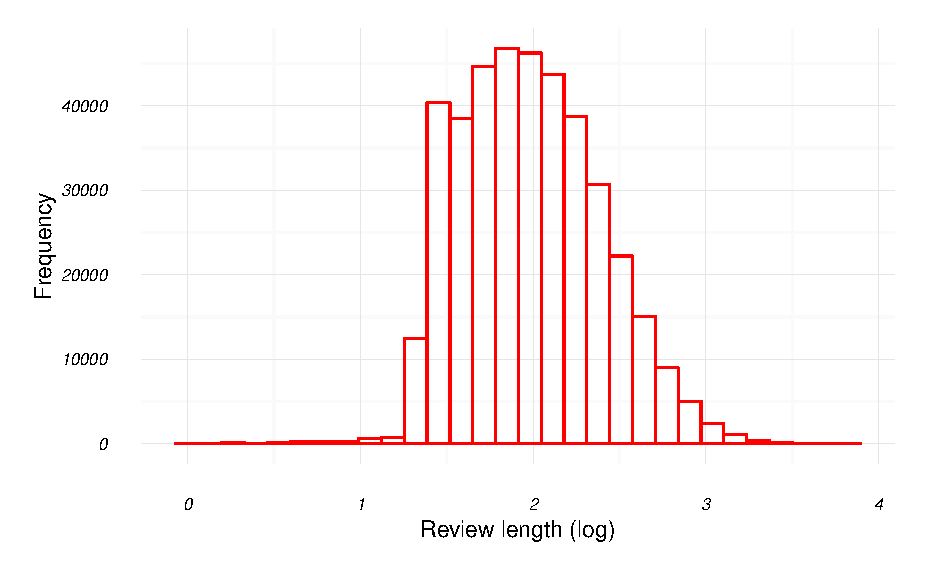
\includegraphics[width=\hsize]{histogram.eps}
  \caption{Distribution of review length.}
  \label{fig_histogram}
\end{figure}

\subsection{Distributed representation approach}
As we have announced above, distributed representation or word embedding method have the explicit advantage of capturing latent semantic relations, so firstly we use word or sentence features extracted from {\itshape word2vec} and {\itshape doc2vec} and then apply them to sentiment classification tasks through a simple neural network. A typical structure of neural networks we adopted here is shown in Figure~\ref{fig_neural}.

\begin{figure}[tb]
  \centering
  \vspace{0.2cm}
  \includegraphics[width=\hsize]{neural1.pdf}
  \caption{A typical structure of neural networks.}
  \label{fig_neural}
\end{figure}

\subsubsection{Word vector averaging}
%\textbf{Word vector averaging.}
Firstly, with the aid of {\itshape word2vec}, a given word is represented by a vector with a reasonable dimension (tens to hundreds, according to the specification assigned to it). In our case, we adopt 320 000 review texts and train them to get vectors of words with a dimension of 300. For example, given a word `{\em sun}', it can be represented by a 300 dimensional vector, say $v(`sun')=[v_1,v_2,\ldots,v_{300}]$. Then, for a given sentence we can get the corresponding vector easily by averaging the word vectors in the sentence. 

Note that, to get the average vector of sentence, we neglect stopwords (derived from NLTK\footnote{\href{http://www.nltk.org}{http://www.nltk.org}}.) as many of them don't convey rich information and may even bring in irrelevant influences. We should also notice that for words come form validation set, there may no corresponding existing word vectors because they are out of the vocabulary of train set, so in this scenario we neglect new words as well when computing sentence or paragraph-level vectors.
After we get vectors corresponding to each review, we feed them to neural networks with one hidden layer to do classification tasks with the aid of {\itshape Tensorflow}, and the primary result of 5-way classification is shown in Table~\ref{tab1}.  Beyond that, we also conduct some additional experiment between different combination of classes, part of results are show in Appendix. 

\subsubsection{Paragraph vector}
%\textbf{Paragraph vector.}
Paragraph vector or {\itshape doc2vec} works in a way similar with {\itshape word2vec}, but the superior is that we can get the paragraph-level vector directly, which will liberate labors greatly. In the same way, we conduct sentiment classification tasks by training review vectors through a typical neural network with one layer. Result is reported in Table~\ref{tab1}, obviously, we don't get a higher accuracy as expected. The reason may be that paragraph vector learned in Le et al. \cite{le2014distributed} contains two types of vectors: one learned by the standard paragraph vector with distributed memory (PV-DM) and the other learned by the paragraph vector with distributed bag-of-words (PV- DBOW), but in our study we only take PV-DM into consideration which may lose many rich information. In addition, they have made use of  unlabeled data to train the model ,which may help a lot to distinguish boundaries between different classes in classification task, while we don't leverage any other data to train our model.

\subsubsection{FastText}
%\textbf{ FastText.} 
 {\itshape FastText} works in a way similar with  {\itshape word2vec} while taking local word order into consideration \cite{bojanowski2016enriching, joulin2016bag}. Result in Table~\ref{tab1} shows that it can really achieve good performance compared with the other two word embedding methods. Moreover, as  {\itshape fastText} is implemented in C++, as such it works fast indeed just as its name implies: in our task, only 1 minute is needed for the main function to get an accuracy of about 55\% in five-way classification task.

\begin{table}
\centering
\caption{Results of sentiment classification tasks.}
\label{tab1}
\begin{tabular}{|c|c|l|} \hline
Method&Accuracy for 5-way classification \\ \hline
Word vector averaging & 47.3\% \\ \hline
Paragraph vector & 30.8 \% \\ \hline
{\itshape fastText} & 55.7 \% \\ \hline
LSTM & 54.3 \% \\ \hline
%\$ & 4 in 5 & Used in business\\ \hline
%$\Psi^2_1$ & 1 in 40,000& Unexplained usage\\
\end{tabular}
\end{table}

\subsection{Recurrent neural network approach}
In our project, we mainly conduct experiment on  LSTM (long short-term memory) architecture. Firstly, words are processed and mapped into a unique and distinct id, however, troublesome problem occurs consequently, as there are many typos in the review data resulting in a high dimensional word space. To remedy this, we only chose top 10 000 words by their term frequency in the data. Note that, 10 000 words in english corpus are enough to help us capture the word information while training more efficient as it reduces possible word space. 

Classification result in Table~\ref{tab1} shows that LSTM achieves significant improvement compared with word vector averaging or paragraph vector approaches but performs slightly poorly when compared with  {\itshape FastText}. Generally, Recurrent Neural Networks are difficult to train, especially for people without professional knowledge of RNN, this may be the main reason  in this scenario. Furthermore, due to limitation we just train RNN for several Iterative steps, which may be not enough to get a striking result.

\section{DISCUSSION AND CONCLUSIONS}
In our project, we investigate sentiment analysis through several approaches, including word vector averaging, paragraph vector, {\itshape fasetText} and LSTM. Different from previous studies, where datasets used are fine-gained or only contain two classes (i.e., positive and negative), dataset adopted in our study is randomly selected from raw review data and of variable text length. Experiments show that RNN/LSTM performs better than simple word embedding methods like {\itshape word2vec}, {\itshape doc2vec}, but when taking local word order into consideration, just as  {\itshape fasetText} states, word embedding method can achieve competitive results compared with RNN/LSTM. 

In addition, since PCA could decompose matrix into certain length while keeping the major information of the matrix, we also conduct a matrix factorization which is just the exact representation of quantified words, we put the vector of words as columns sequentially.  And then we did the PCA decomposition with 4 components left, however we don't achieve expected results. This direction still needs to explore.

Taken together, through this project we recognize the amazing power of word embedding and neural networks. We still need to learn more in Big Data Analytics in this era of Big Data.

%\begin{picture}(100,100)
%\put(0,0){\includegraphics{....}}
%\put(10,10){hello}

%\begin{figure}
%\centering
%\includegraphics{flies}
%\caption{A sample black and white graphic.}
%\end{figure}
%
%\begin{figure*}
%\centering
%\includegraphics{flies}
%\caption{A sample black and white graphic
%that needs to span two columns of text.}
%\end{figure*}
%
%\section{The {\secit Body} of The Paper}
%Typically, the body of a paper is organized
%into a hierarchical structure, with numbered or unnumbered
%headings for sections, subsections, sub-subsections, and even
%smaller sections.  The command \texttt{{\char'134}section} that
%precedes this paragraph is part of such a
%hierarchy.\footnote{This is the second footnote.  It
%starts a series of three footnotes that add nothing
%informational, but just give an idea of how footnotes work
%and look. It is a wordy one, just so you see
%how a longish one plays out.} \LaTeX\ handles the numbering
%and placement of these headings for you, when you use
%the appropriate heading commands around the titles
%of the headings.  If you want a sub-subsection or
%smaller part to be unnumbered in your output, simply append an
%asterisk to the command name.  Examples of both
%numbered and unnumbered headings will appear throughout the
%balance of this sample document.
%
%Because the entire article is contained in
%the \textbf{document} environment, you can indicate the
%start of a new paragraph with a blank line in your
%input file; that is why this sentence forms a separate paragraph.
%
%\subsection{Type Changes and {\subsecit Special} Characters}
%We have already seen several typeface changes in this sample.  You
%can indicate italicized words or phrases in your text with
%the command \texttt{{\char'134}textit}; emboldening with the
%command \texttt{{\char'134}textbf}
%and typewriter-style (for instance, for computer code) with
%\texttt{{\char'134}texttt}.  But remember, you do not
%have to indicate typestyle changes when such changes are
%part of the \textit{structural} elements of your
%article; for instance, the heading of this subsection will
%be in a sans serif\footnote{A third footnote, here.
%Let's make this a rather short one to
%see how it looks.} typeface, but that is handled by the
%document class file. Take care with the use
%of\footnote{A fourth, and last, footnote.}
%the curly braces in typeface changes; they mark
%the beginning and end of
%the text that is to be in the different typeface.
%
%You can use whatever symbols, accented characters, or
%non-English characters you need anywhere in your document;
%you can find a complete list of what is
%available in the \textit{\LaTeX\
%User's Guide}\cite{Lamport:LaTeX}.
%
%\subsection{Math Equations}
%You may want to display math equations in three distinct styles:
%inline, numbered or non-numbered display.  Each of
%the three are discussed in the next sections.
%
%\subsubsection{Inline (In-text) Equations}
%A formula that appears in the running text is called an
%inline or in-text formula.  It is produced by the
%\textbf{math} environment, which can be
%invoked with the usual \texttt{{\char'134}begin. . .{\char'134}end}
%construction or with the short form \texttt{\$. . .\$}. You
%can use any of the symbols and structures,
%from $\alpha$ to $\omega$, available in
%\LaTeX\cite{Lamport:LaTeX}; this section will simply show a
%few examples of in-text equations in context. Notice how
%this equation: \begin{math}\lim_{n\rightarrow \infty}x=0\end{math},
%set here in in-line math style, looks slightly different when
%set in display style.  (See next section).
%
%\subsubsection{Display Equations}
%A numbered display equation -- one set off by vertical space
%from the text and centered horizontally -- is produced
%by the \textbf{equation} environment. An unnumbered display
%equation is produced by the \textbf{displaymath} environment.
%
%Again, in either environment, you can use any of the symbols
%and structures available in \LaTeX; this section will just
%give a couple of examples of display equations in context.
%First, consider the equation, shown as an inline equation above:
%\begin{equation}\lim_{n\rightarrow \infty}x=0\end{equation}
%Notice how it is formatted somewhat differently in
%the \textbf{displaymath}
%environment.  Now, we'll enter an unnumbered equation:
%\begin{displaymath}\sum_{i=0}^{\infty} x + 1\end{displaymath}
%and follow it with another numbered equation:
%\begin{equation}\sum_{i=0}^{\infty}x_i=\int_{0}^{\pi+2} f\end{equation}
%just to demonstrate \LaTeX's able handling of numbering.

%\subsection{Citations}
%Citations to articles \cite{bowman:reasoning,
%clark:pct, braams:babel, herlihy:methodology},
%conference proceedings \cite{clark:pct} or
%books \cite{salas:calculus, Lamport:LaTeX} listed
%in the Bibliography section of your
%article will occur throughout the text of your article.
%You should use BibTeX to automatically produce this bibliography;
%you simply need to insert one of several citation commands with
%a key of the item cited in the proper location in
%the \texttt{.tex} file \cite{Lamport:LaTeX}.
%The key is a short reference you invent to uniquely
%identify each work; in this sample document, the key is
%the first author's surname and a
%word from the title.  This identifying key is included
%with each item in the \texttt{.bib} file for your article.
%
%The details of the construction of the \texttt{.bib} file
%are beyond the scope of this sample document, but more
%information can be found in the \textit{Author's Guide},
%and exhaustive details in the \textit{\LaTeX\ User's
%Guide}\cite{Lamport:LaTeX}.
%
%This article shows only the plainest form
%of the citation command, using \texttt{{\char'134}cite}.
%This is what is stipulated in the SIGS style specifications.
%No other citation format is endorsed or supported.
%
%\subsection{Tables}
%Because tables cannot be split across pages, the best
%placement for them is typically the top of the page
%nearest their initial cite.  To
%ensure this proper ``floating'' placement of tables, use the
%environment \textbf{table} to enclose the table's contents and
%the table caption.  The contents of the table itself must go
%in the \textbf{tabular} environment, to
%be aligned properly in rows and columns, with the desired
%horizontal and vertical rules.  Again, detailed instructions
%on \textbf{tabular} material
%is found in the \textit{\LaTeX\ User's Guide}.
%
%Immediately following this sentence is the point at which
%Table 1 is included in the input file; compare the
%placement of the table here with the table in the printed
%dvi output of this document.
%
%\begin{table}
%\centering
%\caption{Frequency of Special Characters}
%\begin{tabular}{|c|c|l|} \hline
%Non-English or Math&Frequency&Comments\\ \hline
%\O & 1 in 1,000& For Swedish names\\ \hline
%$\pi$ & 1 in 5& Common in math\\ \hline
%\$ & 4 in 5 & Used in business\\ \hline
%$\Psi^2_1$ & 1 in 40,000& Unexplained usage\\
%\hline\end{tabular}
%\end{table}
%
%To set a wider table, which takes up the whole width of
%the page's live area, use the environment
%\textbf{table*} to enclose the table's contents and
%the table caption.  As with a single-column table, this wide
%table will ``float" to a location deemed more desirable.
%Immediately following this sentence is the point at which
%Table 2 is included in the input file; again, it is
%instructive to compare the placement of the
%table here with the table in the printed dvi
%output of this document.
%
%
%\begin{table*}
%\centering
%\caption{Some Typical Commands}
%\begin{tabular}{|c|c|l|} \hline
%Command&A Number&Comments\\ \hline
%\texttt{{\char'134}alignauthor} & 100& Author alignment\\ \hline
%\texttt{{\char'134}numberofauthors}& 200& Author enumeration\\ \hline
%\texttt{{\char'134}table}& 300 & For tables\\ \hline
%\texttt{{\char'134}table*}& 400& For wider tables\\ \hline\end{tabular}
%\end{table*}
%% end the environment with {table*}, NOTE not {table}!
%
%\subsection{Figures}
%Like tables, figures cannot be split across pages; the
%best placement for them
%is typically the top or the bottom of the page nearest
%their initial cite.  To ensure this proper ``floating'' placement
%of figures, use the environment
%\textbf{figure} to enclose the figure and its caption.
%
%This sample document contains examples of \textbf{.eps} files to be
%displayable with \LaTeX.  If you work with pdf\LaTeX, use files in the
%\textbf{.pdf} format.  Note that most modern \TeX\ system will convert
%\textbf{.eps} to \textbf{.pdf} for you on the fly.  More details on
%each of these is found in the \textit{Author's Guide}.
%
%\begin{figure}
%\centering
%\includegraphics{fly}
%\caption{A sample black and white graphic.}
%\end{figure}
%
%\begin{figure}
%\centering
%\includegraphics[height=1in, width=1in]{fly}
%\caption{A sample black and white graphic
%that has been resized with the \texttt{includegraphics} command.}
%\end{figure}
%
%
%As was the case with tables, you may want a figure
%that spans two columns.  To do this, and still to
%ensure proper ``floating'' placement of tables, use the environment
%\textbf{figure*} to enclose the figure and its caption.
%and don't forget to end the environment with
%{figure*}, not {figure}!
%
%\begin{figure*}
%\centering
%\includegraphics{flies}
%\caption{A sample black and white graphic
%that needs to span two columns of text.}
%\end{figure*}
%
%
%\begin{figure}
%\centering
%\includegraphics[height=1in, width=1in]{rosette}
%\caption{A sample black and white graphic that has
%been resized with the \texttt{includegraphics} command.}
%\vskip -6pt
%\end{figure}
%
%\subsection{Theorem-like Constructs}
%Other common constructs that may occur in your article are
%the forms for logical constructs like theorems, axioms,
%corollaries and proofs.  There are
%two forms, one produced by the
%command \texttt{{\char'134}newtheorem} and the
%other by the command \texttt{{\char'134}newdef}; perhaps
%the clearest and easiest way to distinguish them is
%to compare the two in the output of this sample document:
%
%This uses the \textbf{theorem} environment, created by
%the\linebreak\texttt{{\char'134}newtheorem} command:
%\newtheorem{theorem}{Theorem}
%\begin{theorem}
%Let $f$ be continuous on $[a,b]$.  If $G$ is
%an antiderivative for $f$ on $[a,b]$, then
%\begin{displaymath}\int^b_af(t)dt = G(b) - G(a).\end{displaymath}
%\end{theorem}
%
%The other uses the \textbf{definition} environment, created
%by the \texttt{{\char'134}newdef} command:
%\newdef{definition}{Definition}
%\begin{definition}
%If $z$ is irrational, then by $e^z$ we mean the
%unique number which has
%logarithm $z$: \begin{displaymath}{\log e^z = z}\end{displaymath}
%\end{definition}
%
%Two lists of constructs that use one of these
%forms is given in the
%\textit{Author's  Guidelines}.
% 
%There is one other similar construct environment, which is
%already set up
%for you; i.e. you must \textit{not} use
%a \texttt{{\char'134}newdef} command to
%create it: the \textbf{proof} environment.  Here
%is a example of its use:
%\begin{proof}
%Suppose on the contrary there exists a real number $L$ such that
%\begin{displaymath}
%\lim_{x\rightarrow\infty} \frac{f(x)}{g(x)} = L.
%\end{displaymath}
%Then
%\begin{displaymath}
%l=\lim_{x\rightarrow c} f(x)
%= \lim_{x\rightarrow c}
%\left[ g{x} \cdot \frac{f(x)}{g(x)} \right ]
%= \lim_{x\rightarrow c} g(x) \cdot \lim_{x\rightarrow c}
%\frac{f(x)}{g(x)} = 0\cdot L = 0,
%\end{displaymath}
%which contradicts our assumption that $l\neq 0$.
%\end{proof}
%
%Complete rules about using these environments and using the
%two different creation commands are in the
%\textit{Author's Guide}; please consult it for more
%detailed instructions.  If you need to use another construct,
%not listed therein, which you want to have the same
%formatting as the Theorem
%or the Definition\cite{salas:calculus} shown above,
%use the \texttt{{\char'134}newtheorem} or the
%\texttt{{\char'134}newdef} command,
%respectively, to create it.
%\cite{duan2008dynamics}
%
%\subsection*{A {\secit Caveat} for the \TeX\ Expert}
%Because you have just been given permission to
%use the \texttt{{\char'134}newdef} command to create a
%new form, you might think you can
%use \TeX's \texttt{{\char'134}def} to create a
%new command: \textit{Please refrain from doing this!}
%Remember that your \LaTeX\ source code is primarily intended
%to create camera-ready copy, but may be converted
%to other forms -- e.g. HTML. If you inadvertently omit
%some or all of the \texttt{{\char'134}def}s recompilation will
%be, to say the least, problematic.
%
%\section{Conclusions}
%This paragraph will end the body of this sample document.
%Remember that you might still have Acknowledgments or
%Appendices; brief samples of these
%follow.  There is still the Bibliography to deal with; and
%we will make a disclaimer about that here: with the exception
%of the reference to the \LaTeX\ book, the citations in
%this paper are to articles which have nothing to
%do with the present subject and are used as
%examples only.
%%\end{document}  % This is where a 'short' article might terminate
%
%%ACKNOWLEDGMENTS are optional
%\section{Acknowledgments}
%This section is optional; it is a location for you
%to acknowledge grants, funding, editing assistance and
%what have you.  In the present case, for example, the
%authors would like to thank Gerald Murray of ACM for
%his help in codifying this \textit{Author's Guide}
%and the \textbf{.cls} and \textbf{.tex} files that it describes.

%
% The following two commands are all you need in the
% initial runs of your .tex file to
% produce the bibliography for the citations in your paper.
\bibliographystyle{abbrv}
\bibliography{Engg5108}  % sigproc.bib is the name of the Bibliography in this case
% You must have a proper ".bib" file
%  and remember to run:
% latex bibtex latex latex
% to resolve all references
%
% ACM needs 'a single self-contained file'!
%
%APPENDICES are optional
\balancecolumns
\appendix

%Appendix A
\begin{table}[h]
\centering
\caption{Sentiment classification results of word vector averaging.}
\label{tab2}
\begin{tabular}{|c|c|l|} \hline
Classification (different classes separated by ',')&Accuracy \\ \hline
123, 45 & 80.0\% \\ \hline
12, 345 & 79.9\%\\ \hline
12, 3, 45 & 68.2\%\\ \hline
1, 2 & 67.6\% \\ \hline
1, 2, 3 & 55.9\% \\ \hline
1, 2, 3, 4, 5 & 47.3\% \\ \hline
1, 5 & 90.0\% \\ \hline
3, 4, 5 & 57.3\% \\ \hline
4, 5 & 69.1\% \\ \hline
\end{tabular}
\end{table}
%
\begin{table}[h]
\centering
\caption{Sentiment classification results of paragraph vector.}
\label{tab3}
\begin{tabular}{|c|c|l|} \hline
Classification (different classes separated by ',')&Accuracy \\ \hline
123, 45 & 64.6\% \\ \hline
12, 345 & 68.5\%\\ \hline
1, 2 & 61.0\% \\ \hline
1, 2, 3 & 45.8\% \\ \hline
1, 2, 3, 4, 5 & 30.8\% \\ \hline
1, 5 & 72.4\% \\ \hline
3, 4, 5 & 40.0\% \\ \hline
4, 5 & 52.9\% \\ \hline\end{tabular}
\end{table}

%\begin{table}[h]
%\centering
%\caption{Tolerant Classification}
%\label{tab4}
%\begin{tabular}{|c|c|cl||||} \hline
%Classification &1&2&3&4&5&Total accuracy \\ \hline
%Normal classification & 61.7\% & 37.8\% & 38.3\% & 67.1\% & 67.1\% & 47.3\% \\ \hline
%Tolerable classification & 85.6\% & 88.0\% & 76.9\% & 87.6\% & 82.5\% & 84.1\% \\ \hline\end{tabular}
%\end{table}

%\begin{table}[h]
%\centering
%\caption{Sentiment classification results of paragraph vector.}
%\label{tab3}
%\begin{tabular}{|c|c|l|} \hline
%Classification (different classes separated by ',')&Accuracy \\ \hline
%123, 45 & 64.6\% \\ \hline
%12, 345 & 68.5\%\\ \hline
%1, 2 & 61.0\% \\ \hline
%1, 2, 3 & 45.8\% \\ \hline
%1, 2, 3, 4, 5 & 30.8\% \\ \hline
%1, 5 & 72.4\% \\ \hline
%3, 4, 5 & 40.0\% \\ \hline
%4, 5 & 52.9\% \\ \hline\end{tabular}
%\end{table}


%
%\section{Headings in Appendices}
%The rules about hierarchical headings discussed above for
%the body of the article are different in the appendices.
%In the \textbf{appendix} environment, the command
%\textbf{section} is used to
%indicate the start of each Appendix, with alphabetic order
%designation (i.e. the first is A, the second B, etc.) and
%a title (if you include one).  So, if you need
%hierarchical structure
%\textit{within} an Appendix, start with \textbf{subsection} as the
%highest level. Here is an outline of the body of this
%document in Appendix-appropriate form:
%\subsection{Introduction}
%\subsection{The Body of the Paper}
%\subsubsection{Type Changes and  Special Characters}
%\subsubsection{Math Equations}
%\paragraph{Inline (In-text) Equations}
%\paragraph{Display Equations}
%\subsubsection{Citations}
%\subsubsection{Tables}
%\subsubsection{Figures}
%\subsubsection{Theorem-like Constructs}
%\subsubsection*{A Caveat for the \TeX\ Expert}
%\subsection{Conclusions}
%\subsection{Acknowledgments}
%\subsection{Additional Authors}
%This section is inserted by \LaTeX; you do not insert it.
%You just add the names and information in the
%\texttt{{\char'134}additionalauthors} command at the start
%of the document.
%\subsection{References}
%Generated by bibtex from your ~.bib file.  Run latex,
%then bibtex, then latex twice (to resolve references)
%to create the ~.bbl file.  Insert that ~.bbl file into
%the .tex source file and comment out
%the command \texttt{{\char'134}thebibliography}.
%% This next section command marks the start of
%% Appendix B, and does not continue the present hierarchy
%\section{More Help for the Hardy}
%The sig-alternate.cls file itself is chock-full of succinct
%and helpful comments.  If you consider yourself a moderately
%experienced to expert user of \LaTeX, you may find reading
%it useful but please remember not to change it.
%\balancecolumns % GM June 2007
% That's all folks!
%\bibliographystyle{abbrv}
%\bibliography{sigproc}
\end{document}
